\documentclass[12pt,letterpaper]{article}
\usepackage[utf8]{inputenc}
\usepackage[spanish]{babel}
\usepackage{graphicx}
\usepackage[left=2cm,right=2cm,top=2cm,bottom=2cm]{geometry}
\usepackage{graphicx} % figuras
% \usepackage{subfigure} % subfiguras
\usepackage{float} % para usar [H]
\usepackage{amsmath}
%\usepackage{txfonts}
\usepackage{stackrel} 
\usepackage{multirow}
\usepackage{enumerate} % enumerados
\renewcommand{\labelitemi}{$-$}
\renewcommand{\labelitemii}{$\cdot$}
% \author{}
% \title{Caratula}
\begin{document}

% Fancy Header and Footer
% \usepackage{fancyhdr}
% \pagestyle{fancy}
% \cfoot{}
% \rfoot{\thepage}
%

% \usepackage[hidelinks]{hyperref} % CREA HYPERVINCULOS EN INDICE

% \author{}
\title{Caratula}

\begin{titlepage}
\begin{center}
\large{UNIVERSIDAD PRIVADA DE TACNA}\\
\vspace*{-0.025in}
\begin{figure}[htb]
\begin{center}

\includegraphics[width=8cm]{./Imagenes/logo}
\end{center}
\end{figure}
\vspace*{0.15in}
INGENIERIA DE SISTEMAS  \\

\vspace*{0.5in}
\begin{large}
TITULO:\\
\end{large}

\vspace*{0.1in}
\begin{Large}
\textbf{TRABAJO DE INVESTIGACI\'ON} \\
\end{Large}

\vspace*{0.3in}
\begin{Large}
\textbf{CURSO:} \\
\end{Large}

\vspace*{0.1in}
\begin{large}
BASE DE DATOS II\\
\end{large}

\vspace*{0.3in}
\begin{Large}
\textbf{DOCENTE(ING):} \\
\end{Large}

\vspace*{0.1in}
\begin{large}
 Patrick Cuadros Quiroga\\
\end{large}

\vspace*{0.2in}
\vspace*{0.1in}
\begin{large}
Alumno: \\
\begin{flushleft}
Katerin Almendra MERINO QUISPE\hfill	(2018060918) \\
\end{flushleft}
\end{large}
\end{center}

\end{titlepage}


\tableofcontents % INDICE
\thispagestyle{empty} % INDICE SIN NUMERO
\newpage
\setcounter{page}{1} % REINICIAR CONTADOR DE PAGINAS DESPUES DEL INDICE



\begin{Large}
\begin{center}
\textbf{Control de versiones} \\
\end{center}
\end{Large}

\section{Control de versiones} 
Se llama control de versiones a la gestión de los diversos cambios que se realizan sobre los elementos de algún producto o una configuración del mismo. Una versión, revisión o edición de un producto, es el estado en el que se encuentra el mismo en un momento dado de su desarrollo o modificación.

Aunque un sistema de control de versiones puede realizarse de forma manual, es muy aconsejable disponer de herramientas que faciliten esta gestión dando lugar a los llamados sistemas de control de versiones o VCS (del inglés Version Control System). Estos sistemas facilitan la administración de las distintas versiones de cada producto desarrollado, así como las posibles especializaciones realizadas (por ejemplo, para algún cliente específico). Ejemplos de este tipo de herramientas son entre otros: CVS, Subversion, SourceSafe, ClearCase, Darcs, Bazaar, Plastic SCM, Git, SCCS, Mercurial, Perforce, Fossil SCM, Team Foundation Server.

\begin{itemize}
	\begin{center}
	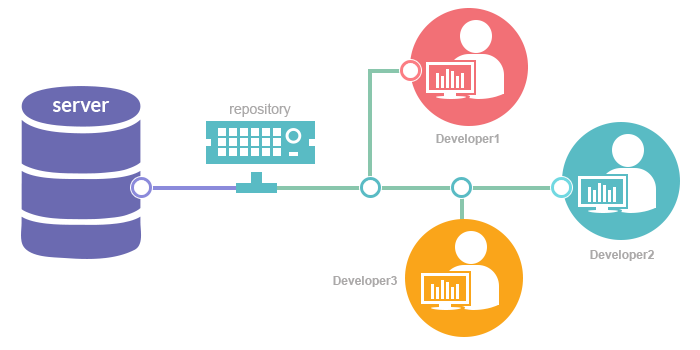
\includegraphics[width=14cm]{./Imagenes/imagen2} 
	\end{center}

	\item Si eres diseñador gráfico o web, y quieres mantener cada versión de una imagen o diseño (algo que sin duda quieres), un sistema de control de versiones (Version Control System o VCS en inglés) es una elección muy sabia. Te permite revertir archivos a un estado anterior, revertir el proyecto entero a un estado anterior, comparar cambios a lo largo del tiempo, ver quién modificó por última vez algo que puede estar causando un problema, quién introdujo un error y cuándo, y mucho más. Usar un VCS también significa generalmente que si fastidias o pierdes archivos, puedes recuperarlos fácilmente. Además, obtienes todos estos beneficios a un coste muy bajo.



\end{itemize} 

\section{Sistemas de control de versiones locales} 
Un método de control de versiones usado por mucha gente es copiar los archivos a otro directorio (quizás indicando la fecha y hora en que lo hicieron, si son avispados). Este enfoque es muy común porque es muy simple, pero también tremendamente propenso a errores. Es fácil olvidar en qué directorio te encuentras, y guardar accidentalmente en el archivo equivocado o sobrescribir archivos que no querías.

\begin{itemize}
	\begin{center}
	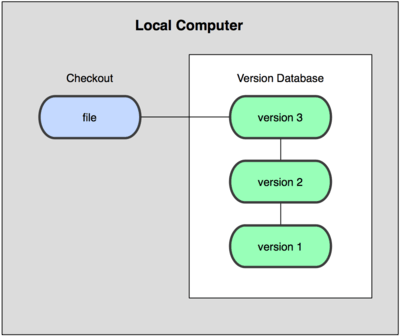
\includegraphics[width=14cm]{./Imagenes/imagen3} 
	\end{center}

	\item Una de las herramientas de control de versiones más popular fue un sistema llamado rcs, que todavía podemos encontrar en muchos de los ordenadores actuales. Hasta el famoso sistema operativo Mac OS X incluye el comando rcs cuando instalas las herramientas de desarrollo. Esta herramienta funciona básicamente guardando conjuntos de parches (es decir, las diferencias entre archivos) de una versión a otra en un formato especial en disco; puede entonces recrear cómo era un archivo en cualquier momento sumando los distintos parches.



\end{itemize} 
\section{Sistemas de control de versiones centralizados} 
El siguiente gran problema que se encuentra la gente es que necesitan colaborar con desarrolladores en otros sistemas. Para solventar este problema, se desarrollaron los sistemas de control de versiones centralizados (Centralized Version Control Systems o CVCSs en inglés). Estos sistemas, como CVS, Subversion, y Perforce, tienen un único servidor que contiene todos los archivos versionados, y varios clientes que descargan los archivos desde ese lugar central. Durante muchos años éste ha sido el estándar para el control de versiones

\begin{itemize}
	\begin{center}
	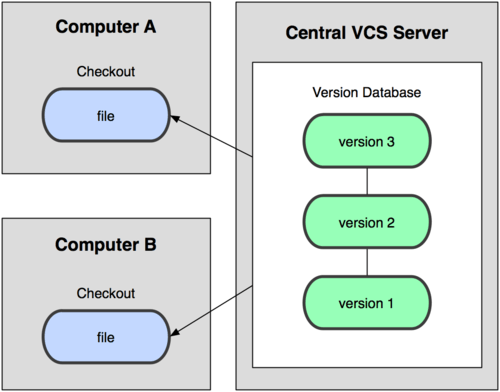
\includegraphics[width=14cm]{./Imagenes/imagen4} 
	\end{center}

	\item Esta configuración ofrece muchas ventajas, especialmente frente a VCSs locales. Por ejemplo, todo el mundo puede saber (hasta cierto punto) en qué están trabajando los otros colaboradores del proyecto. Los administradores tienen control detallado de qué puede hacer cada uno; y es mucho más fácil administrar un CVCS que tener que lidiar con bases de datos locales en cada cliente.



\end{itemize} 
\section{Sistemas de control de versiones distribuidos} 
Es aquí donde entran los sistemas de control de versiones distribuidos (Distributed Version Control Systems o DVCSs en inglés). En un DVCS (como Git, Mercurial, Bazaar o Darcs), los clientes no sólo descargan la última instantánea de los archivos: replican completamente el repositorio. Así, si un servidor muere, y estos sistemas estaban colaborando a través de él, cualquiera de los repositorios de los clientes puede copiarse en el servidor para restaurarlo. Cada vez que se descarga una instantánea, en realidad se hace una copia de seguridad completa de todos los datos.

\begin{itemize}
	\begin{center}
	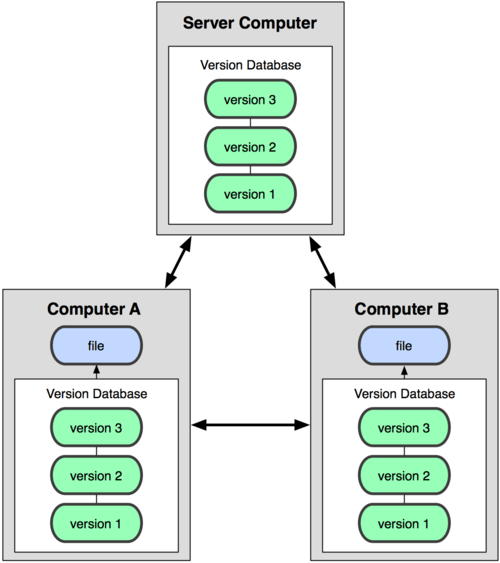
\includegraphics[width=14cm]{./Imagenes/imagen5} 
	\end{center}

	\item Es más, muchos de estos sistemas se las arreglan bastante bien teniendo varios repositorios con los que trabajar, por lo que puedes colaborar con distintos grupos de gente simultáneamente dentro del mismo proyecto. Esto te permite establecer varios flujos de trabajo que no son posibles en sistemas centralizados, como pueden ser los modelos jerárquicos.



\end{itemize} 
\section{Github} 
GitHub es una forja (plataforma de desarrollo colaborativo) para alojar proyectos utilizando el sistema de control de versiones Git. Se utiliza principalmente para la creación de código fuente de programas de computadora. El software que opera GitHub fue escrito en Ruby on Rails. Desde enero de 2010, GitHub opera bajo el nombre de GitHub, Inc. Anteriormente era conocida como Logical Awesome LLC. El código de los proyectos alojados en GitHub se almacena típicamente de forma pública, aunque utilizando una cuenta de pago, también permite hospedar repositorios privados.
\begin{itemize}
	\begin{center}
	
\includegraphics[width=5cm]{./Imagenes/imagen1} 
	\end{center}
\end{itemize}


\section{¿Qué ofrece Github?} \\

Github ofrece al desarrollador toda la potencia y agilidad del sistema de control de versiones Git, más un interesante set de herramientas añadidas:
Wiki
Sistema de seguimiento de incidencias
Interfaz gráfica para revisión/comparación de código
Visor de ramas de desarrollo. \\


\section{¿Cómo funciona Github?} \\

Lo primero que debemos hacer es crear una cuenta en https://github.com. La activamos por mail y ya podemos crear nuestros repositorios. Los repositorios de Github son el almacén que utilizamos para guardar nuestro código. Github nos ofrece la opción de crear un repositorio vacío, recomendable cuando vamos a iniciar un nuevo desarrollo, o la opción de importar un proyecto ya existente, elegimos la que más nos convenga y mediante unos pocos comandos de consola configuramos la rama principal de nuestro repositorio, que por defecto se llamará "master". Cada programador puede crear sus propias ramas de desarrollo, donde tiene que llevar a cabo sus modificaciones, sin interferir en el trabajo de sus compañeros. Cuando terminamos y validamos un desarrollo paralelo, lo unimos con la rama principal y todos los miembros del equipo pueden descargar las nuevas modificaciones, sin alterar los desarrollos que estén llevando cabo en ese momento. Después de alojar el repositorio público en Github.com, cualquier usuario de la comunidad podrá aportar ideas, hacer un seguimiento del proyecto, incluso copiarlo y modificarlo a su gusto bajo la misma licencia.



\section{GitLab} 
Gitlab es un servicio web de control de versiones y desarrollo de software colaborativo basado en Git. Además de gestor de repositorios, el servicio ofrece también alojamiento de wikis y un sistema de seguimiento de errores, todo ello publicado bajo una Licencia de código abierto.
Fue escrito por los programadores ucranianos Dmitriy Zaporozhets y Valery Sizov en el lenguaje de programación Ruby. La compañía, GitLab Inc., cuenta con un equipo de 150 miembros1​ y más de 1400 usuarios.2​ Es usado por organizaciones como la NASA, el CERN, IBM o Sony.
\begin{itemize}
	\begin{center}
	
\includegraphics[width=5cm]{./Imagenes/imagen6} 
	\end{center}
\end{itemize} 
Como comentan en The Next Web, GitLab es como GitHub pero en esteroides. Es un servicio que también ofrece alojamiento de repositorios con varias funciones de seguimientos de problemas, pero además tiene características extra.

GitLab fue fundado en 2011, y como cuentan ellos mismos, inició como un proyecto en GitHub. A diferencia de este último, en GitLab usan una aplicación única creada desde cero para dar soporte al ciclo entero de desarrollo, en lugar de integrar múltiples herramientas diferentes.\\



\section{GitLab no es un simple clon de GitHub} \\

También tiene un plan básico gratuito que permite aprovechar la plataforma para construir y ejecutar tus aplicaciones. Y, están aprovechando este momento para ofrecer 75% de descuento en sus planes Gold y Ultimate a los nuevos usuarios.

GitLab tampoco es ningún desconocido, múltiples empresas y marcas conocidas lo usan. Y recientemente el proyecto GNOME se mudó a la plataforma justamente porque buscaban simplificar el proceso de colaboración entre sus múltiples contribuidores. La misma gente de GNOME explica que GitLab no es un simple clon de GitHub.


\end{document}
